\section{Descrizione architettura}
\label{descrizione_architettura}

\subsection{Premesse}
Si procederà alla descrizione dell'architettura realizzata, utilizzando un approccio di tipo top-down, ovvero iniziando da una panoramica delle componenti macroscopiche, per arrivare poi a considerare le componenti più specifiche. Di conseguenza, verranno descritti i package\glossario{} ed i componenti macroscopici per entrare successivamente nel dettaglio delle singole classi, specificando per ognuna: una breve descrizione, il contesto di utilizzo, le dipendenze entranti e/o uscenti e le eventuali classi da cui eredita.
Verranno successivamente messi in rilievo gli utilizzi dei Design Pattern\glossario{} all'interno dell'architettura del sistema, dando una spiegazione più dettagliata degli stessi, in appendice \ref{DDP}.\\
Per i diagrammi dei package\glossario{}, delle classi e di attività, è stato utilizzato lo standard UML\glossario{} 2.0. Nei diagrammi dei package\glossario{} si è fatto uso, ove ritenuto necessario, di colori diversi per migliorare la leggibilità dei diversi componenti.\\
Si è deciso di separare le View dai rispettivi Controller, in quanto è emersa la volontà di separare maggiormente la rappresentazione grafica della View dalla propria gestione degli eventi.
Si fornisce di seguito una breve legenda dei colori utilizzati per le package\glossario{} e classi in particolare:
\begin{itemize}
\item Per i package\g{}:
\begin{itemize}
\item \textbf{sfondo bianco con bordo in grassetto:} per identificare il package\g{} Romeo che contiene l'intera architettura;
\item \textbf{sfondo giallo con bordo nero:} per identificare il package\g{} Model che contiene la logica di business; 
\item \textbf{sfondo verde smeraldo con bordo nero:} per identificare il package\g{} View che contiene le componenti grafiche dell'applicativo;
\item \textbf{sfondo arancio con bordo nero:} per identificare il package\g{} Controller che contiene tutti i meccanismi per far far comunicare indirettamente logica di business e logica di presentazione;
\item \textbf{sfondo più chiaro con bordo nero:} per identificare i sotto-package\g{} contenuti nei package\g{} principali (model, view e controller); ad ogni livello il colore si attenua.
\end{itemize}
\item Per le classi:
\begin{itemize}
	\item \textbf{sfondo giallo chiaro con bordo rosso:} per identificare le classi proprie dell'applicativo \project{};
	\item \textbf{sfondo verde acceso con bordo nero:} per identificare le classi di Qt\g{} che verranno utilizzate per realizzare \project{};
	\item \textbf{sfondo blu chiaro con bordo nero:} per identificare le classi di ITK\g{} che verranno utilizzate per realizzare \project{}.
\end{itemize}
\end{itemize}

\pagebreak

\subsection{Architettura generale}
\label{arch_generica}
	L'architettura del software segue quanto stabilito dal design pattern\glossario{} MVC\glossario{}, ed è quindi suddivisa nelle seguenti parti:
	\begin{itemize}
		\item \textbf{Model:} rappresenta la logica di \emph{business};
		\item \textbf{View:} visualizza i dati all'utente;
		\item \textbf{Controller:} rappresenta la logica \emph{applicativa}.
	\end{itemize}
	Nella seguente figura viene presentata l'architettura ad alto livello dell'applicazione, indicando i vari package\glossario{} e le varie relazioni, ad alto livello, tra di loro.
	\begin{figure}[!h]
		\centering
		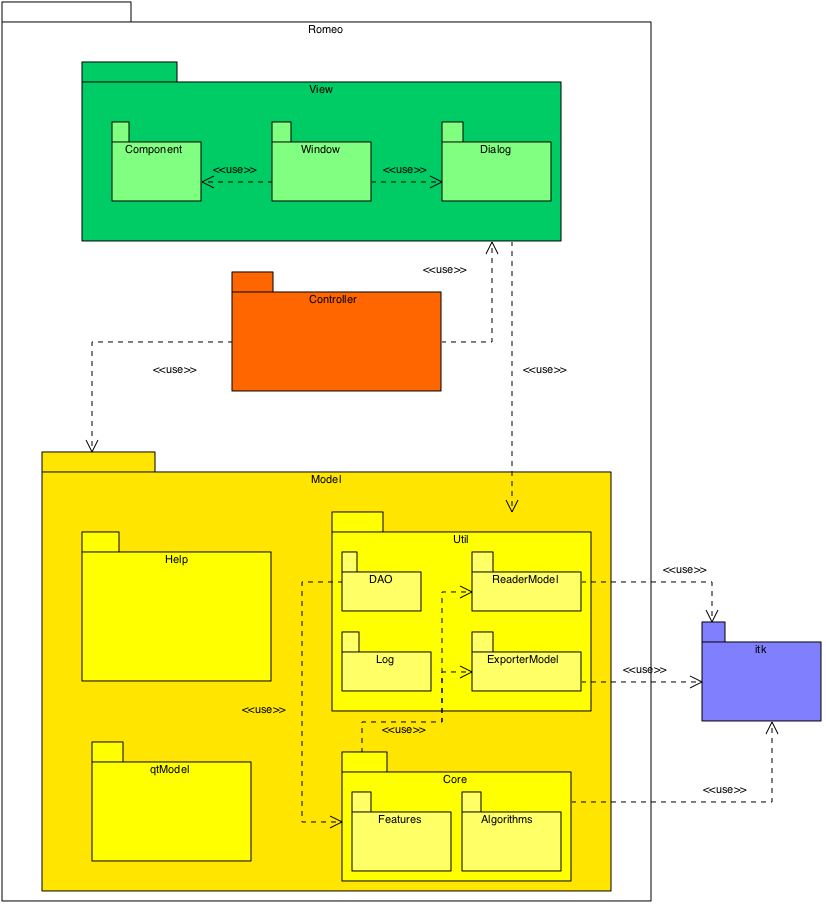
\includegraphics[scale=0.7]{./Content/Immagini/Arch.png}
		\caption{Vista package dell'architettura di \project{}}
		\label{arch_generale}
	\end{figure}
	
	
		
		\begin{landscape}
			\subsubsection{Controller}
			\label{vista_controller}
			\begin{figure}[!h]
				\centering
				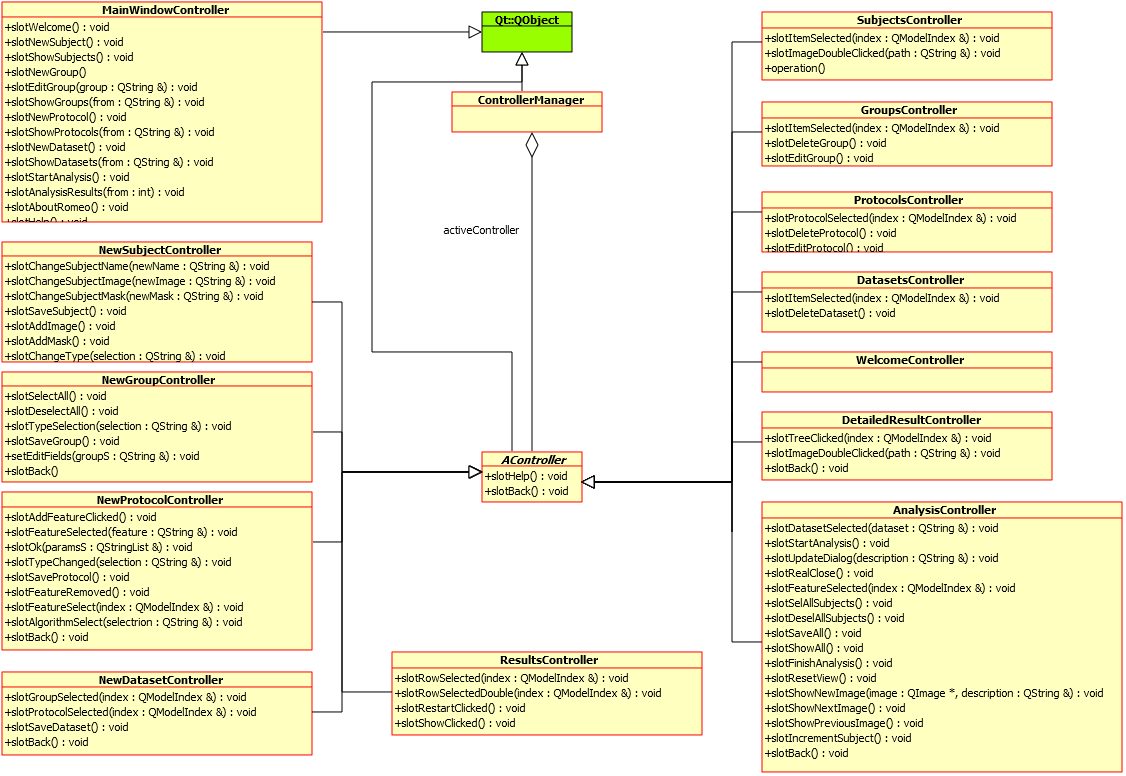
\includegraphics[scale=0.50]{./Content/Immagini/Controller.png}
				\caption{Diagrammi delle classi del componente controller}
				\label{img_controller}
			\end{figure}
		\end{landscape}
		Nel diagramma della classi precedente sono illustrati tutti gli slot presenti nelle classi del package\g{} Controller.
		\\I vari controller ricevono i vari signal\g{} emessi dalla view e hanno il compito di gestirli.
		\\Ogni controller può:
			\begin{itemize}
				\item Aggiornare i dati visualizzati dalla rispettiva view;
				\item Modificare i dati del model;
				\item Aprire nuove view.
			\end{itemize}